% =====================================================================
%  FL-ADTCN — WORK REPORT
%  Paper-extension phase, 30 August – 5 September 2026
%  Build:  pdflatex -interaction=nonstopmode WORK_REPORT.tex   (run twice)
% =====================================================================
\documentclass[11pt]{article}
\usepackage[a4paper,margin=2.2cm,headsep=10pt]{geometry}
\usepackage{microtype}
\usepackage{enumitem}
\usepackage{xcolor}
\usepackage{titlesec}
\usepackage{tabularx}
\usepackage{xltabular}
\usepackage{booktabs}
\usepackage{array}
\usepackage{multirow}
\usepackage{graphicx}
\usepackage[most]{tcolorbox}
\usepackage{tikz}
\usetikzlibrary{arrows.meta,positioning,fit,backgrounds,calc,shapes.geometric,shadows.blur}
\usepackage{fancyhdr}
\usepackage[hidelinks]{hyperref}
\usepackage{parskip}

% ---------------------------------------------------------------- palette
\definecolor{ink}{HTML}{16181D}
\definecolor{navy}{HTML}{1F3A5F}
\definecolor{steel}{HTML}{5A6B7D}
\definecolor{rule}{HTML}{C8CFD8}
\definecolor{wash}{HTML}{F4F6F9}
\definecolor{okgreen}{HTML}{1E6B45}
\definecolor{badred}{HTML}{9B2226}
\definecolor{amber}{HTML}{8A5A00}
\definecolor{lilac}{HTML}{5B4B8A}

\hypersetup{pdftitle={FL-ADTCN Work Report},pdfauthor={Shadman Sakib},
            linkcolor=navy,colorlinks=false}

% ---------------------------------------------------------------- headings
\titleformat{\section}{\Large\bfseries\color{navy}}{\thesection.}{0.55em}{}
\titleformat{\subsection}{\normalsize\bfseries\color{ink}}{\thesubsection}{0.6em}{}
\titleformat{\subsubsection}[runin]{\normalsize\bfseries\color{steel}}{}{0em}{}[\;---]
\titlespacing*{\section}{0pt}{2.6ex}{1.1ex}
\titlespacing*{\subsection}{0pt}{2.0ex}{0.7ex}

\setlist[itemize]{leftmargin=1.3em,topsep=3pt,itemsep=3pt,parsep=0pt}
\setlist[enumerate]{leftmargin=1.6em,topsep=3pt,itemsep=3pt,parsep=0pt}

\pagestyle{fancy}
\fancyhf{}
\renewcommand{\headrulewidth}{0.4pt}
\renewcommand{\headrule}{\hbox to\headwidth{\color{rule}\leaders\hrule height \headrulewidth\hfill}}
\fancyhead[L]{\small\color{steel}FL-ADTCN --- Work Report}
\fancyhead[R]{\small\color{steel}Paper extension, 30 Aug -- 5 Sep 2026}
\fancyfoot[C]{\small\color{steel}\thepage}

% ---------------------------------------------------------------- shorthands
\newcommand{\eps}{\ensuremath{\varepsilon}}
\newcommand{\epsst}{\ensuremath{\varepsilon^{\star}}}
\newcommand{\rh}{\ensuremath{\rho}}
\newcommand{\x}{\ensuremath{\times}}
\newcommand{\atleast}{\ensuremath{\ge}}
\newcommand{\dl}{\ensuremath{\Delta}}
\newcommand{\HELD}{\textcolor{okgreen}{\textbf{\small HELD}}}
\newcommand{\WRONG}{\textcolor{badred}{\textbf{\small WRONG}}}
\newcommand{\PART}{\textcolor{amber}{\textbf{\small PARTLY}}}
\newcommand{\OPEN}{\textcolor{steel}{\textbf{\small OPEN}}}
\newcommand{\dash}{\textcolor{rule}{\rule[0.45ex]{1.1em}{0.7pt}}}

% ---------------------------------------------------------------- boxes
\newtcolorbox{decision}[1]{
  enhanced, colback=white, colframe=navy, boxrule=0.9pt, arc=2pt, breakable,
  left=9pt,right=9pt,top=6pt,bottom=6pt,
  title={\small\bfseries DECISION #1}, coltitle=white, colbacktitle=navy,
  fonttitle=\bfseries, attach boxed title to top left={xshift=8pt,yshift=-2mm},
  boxed title style={colback=navy,boxrule=0pt,arc=1pt}}

\newtcolorbox{keybox}[1]{
  enhanced, colback=wash, colframe=rule, boxrule=0.7pt, arc=2pt, breakable,
  left=9pt,right=9pt,top=7pt,bottom=7pt,
  title={#1}, coltitle=ink, colbacktitle=wash,
  fonttitle=\small\bfseries, titlerule=0.4pt,
  toptitle=4pt, bottomtitle=3pt}

\newtcolorbox{warnbox}[1]{
  enhanced, colback=white, colframe=badred, boxrule=1.0pt, arc=2pt, breakable,
  left=9pt,right=9pt,top=7pt,bottom=7pt,
  title={#1}, coltitle=badred, colbacktitle=white,
  fonttitle=\small\bfseries, titlerule=0.4pt,
  toptitle=4pt, bottomtitle=3pt}

\newcommand{\qlabel}[1]{\textbf{\textcolor{navy}{#1}}\;}

% =====================================================================
\begin{document}
\thispagestyle{empty}

\begin{center}
  \vspace*{0.4cm}
  {\footnotesize\color{steel}\textsc{BRAC University \textbullet\ Department of Computer Science and Engineering \textbullet\ Team T2430460}}\\[14pt]
  {\Huge\bfseries\color{navy} How the Work Changed}\\[8pt]
  {\LARGE\color{ink} A work report on the FL-ADTCN paper extension}\\[16pt]
  \begin{minipage}{0.86\textwidth}\centering
  {\large\itshape Blockchain-Integrated Federated Fraud Detection ---\\ what the accepted thesis got right, what it got wrong,\\ and what six days of controlled re-testing changed about both.}
  \end{minipage}\\[20pt]
  {\color{rule}\rule{0.6\textwidth}{0.8pt}}\\[14pt]
  {\normalsize \textbf{Shadman Sakib} (21301566)}\\[3pt]
  {\small with Md. Abrar-ud-doula Amiya \textbullet\ Mahima Islam \textbullet\ Nafi Alif Mahin \textbullet\ Muntasir Mahin Siam}\\[3pt]
  {\small Supervisor: Md. Golam Rabiul Alam}\\[16pt]
  {\small\color{steel}Reporting period: 30 August -- 5 September 2026 \textbullet\ Compiled 5 September 2026}
\end{center}

\vspace{0.8cm}

\begin{keybox}{The report in six sentences}
The thesis was accepted on 13 June 2026 with one genuine contribution, one honest set of negative
results, and one structural weakness: \textbf{every claim it made rested on a single dataset that has no
customer identities}. Over the last six days we added a second dataset, re-ran five of the six title
claims on it, and then --- crucially --- ran a \emph{control} that separated ``the dataset changed'' from
``the federation structure changed''. That control killed our own most quotable new finding, which is
the single most valuable thing that happened in the period. We then audited the hyperparameter search
the framework is named after and found it had been validating on rows it had trained on; we repaired
it, re-ran the search at full deployment budget for 16.3 hours, and \textbf{the negative result about it
survived unchanged}. Nothing in this report inflates a result: three headline claims were withdrawn or
retired in these six days, all three by our own controls rather than by a reviewer. \textbf{The work is
smaller than it looked on 30 August and much harder to argue with.}
\end{keybox}

\vfill
{\footnotesize\color{steel}\noindent Every number in this document traces to a JSON file produced by a
script in this repository. Where a number is not quotable, the document says so and says why.
Appendix~B lists which script produced which result.}

\newpage
\tableofcontents
\newpage

% =====================================================================
\section{What this document is}

This is a work report, not a paper. It is written for two readers: a teammate who needs to pick the
work up, and a supervisor who needs to know what changed and whether to trust it. It reads in order,
as a story: where we stood, what was wrong with where we stood, what we decided to do about it, what
happened, and what that leaves us with.

Three things it deliberately does:

\begin{itemize}
  \item \textbf{It names decisions and who made them.} At several points the work could have gone two
  ways. Those forks are marked in blue boxes, with the question that was asked, the answer chosen, the
  reason, and --- most importantly --- what the answer actually produced, including when it produced
  something worse than the alternative would have.
  \item \textbf{It reports failures as results.} Nine predictions written down before their experiments
  ran turned out wrong. Those nine are the most useful material in the period, and they are printed
  next to their original wording rather than quietly replaced.
  \item \textbf{It marks what may not be quoted.} Several numbers that appear in older drafts and in the
  supervisor brief are now invalid or definition-dependent. Section~\ref{sec:quotable} is the list.
\end{itemize}

\begin{keybox}{Status at a glance, 5 September 2026}
\small
\begin{tabularx}{\linewidth}{@{}p{4.7cm} X@{}}
\toprule
\textbf{Phase} & Thesis accepted 13 June 2026. Paper extension active. Deadline \textbf{19 September 2026} (T--14). \\
\textbf{Datasets} & ULB credit-card (284{,}807 tx, 0.17\% fraud, no customer IDs) \textbf{+} BankSim (594{,}643 tx, 1.211\% fraud, 4{,}112 customers). A third is gated on a go/no-go decision dated 12 September. \\
\textbf{Conditions measured} & Three: ULB/stratified, BankSim/stratified, BankSim/entity-disjoint. The third exists only to separate two effects that used to move together. \\
\textbf{Title claims off the original dataset} & \textbf{Five of six} measured on a second dataset; the sixth group (RL / consensus / blockchain) is dataset-independent by design. \\
\textbf{CPU spent in the period} & Roughly 45 hours of experiments, of which 16.3 h was one deliberately expensive run. \\
\textbf{Claims withdrawn or retired in the period} & \textbf{Three}, all by our own controls: the Krum utility mechanism, ``MC top-1 fails from $n\!\approx\!6$'', and the privacy-budget improvement factor as a headline. \\
\textbf{Code state} & All work committed on branch \texttt{obj13-surrogate-repair}. Before 5 September the entire extension existed only as untracked files. \\
\bottomrule
\end{tabularx}
\end{keybox}

% =====================================================================
\section{The system, in one page}

Before anything else, the unit of work needs to be clear, because a mistake we made ourselves in this
period was judging the whole thesis by one of its components.

\textbf{The unit is FL-ADTCN}, a six-part system, not a classifier. Three banks (Bank A / B / C) each
train a local fraud detector on their own transactions. Nobody's raw data moves. What moves is model
weights, and around that movement sit five more mechanisms: differential privacy on what is shared,
Krum to decide whose weights become the global model, Shapley values to decide who gets paid, a
metaheuristic search to pick the detector's hyperparameters, and a Hyperledger Fabric ledger that
records the payments and elects the round leader by reinforcement learning.

\begin{figure}[h]
\centering
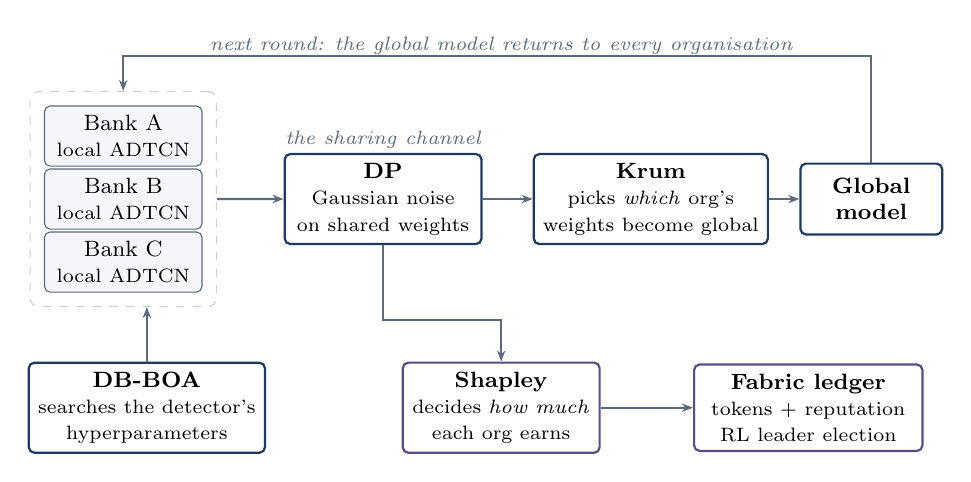
\begin{tikzpicture}[
  font=\footnotesize,
  org/.style={draw=steel,fill=wash,rounded corners=2pt,minimum width=2.0cm,minimum height=0.6cm,align=center},
  proc/.style={draw=navy,fill=white,rounded corners=2pt,minimum width=2.5cm,minimum height=0.9cm,align=center,thick},
  chain/.style={draw=lilac,fill=white,rounded corners=2pt,minimum width=2.5cm,minimum height=0.9cm,align=center,thick},
  ar/.style={-{Stealth[length=4pt]},draw=steel,thick},
  lbl/.style={font=\scriptsize\itshape,text=steel}
]
\node[org] (a) at (1.1,0.0) {Bank A\\\scriptsize local ADTCN};
\node[org] (b) at (1.1,-0.80) {Bank B\\\scriptsize local ADTCN};
\node[org] (c) at (1.1,-1.60) {Bank C\\\scriptsize local ADTCN};
\node[draw=rule,dashed,rounded corners=3pt,fit=(a)(b)(c),inner sep=5pt] (orgbox) {};

\node[proc]                     (dp)    at (4.4,-0.80) {\textbf{DP}\\\scriptsize Gaussian noise\\\scriptsize on shared weights};
\node[proc,minimum width=2.9cm] (krum)  at (7.8,-0.80) {\textbf{Krum}\\\scriptsize picks \emph{which} org's\\\scriptsize weights become global};
\node[proc,minimum width=1.8cm] (glob)  at (10.6,-0.80) {\textbf{Global}\\\textbf{model}};

\node[proc,minimum width=2.7cm] (dbboa) at (1.4,-3.45) {\textbf{DB-BOA}\\\scriptsize searches the detector's\\\scriptsize hyperparameters};
\node[chain]                    (shap)  at (5.9,-3.45) {\textbf{Shapley}\\\scriptsize decides \emph{how much}\\\scriptsize each org earns};
\node[chain,minimum width=2.9cm](ledger) at (9.8,-3.45) {\textbf{Fabric ledger}\\\scriptsize tokens + reputation\\\scriptsize RL leader election};

\draw[ar] (orgbox.east) -- (dp.west);
\node[lbl] at (4.4,-0.04) {the sharing channel};
\draw[ar] (dp) -- (krum);
\draw[ar] (krum) -- (glob);
\draw[ar] (glob.north) -- ++(0,1.35) -| (orgbox.north);
\node[lbl] at (5.9,1.15) {next round: the global model returns to every organisation};
\draw[ar] (dp.south) -- ++(0,-0.95) -| (shap.north);
\draw[ar] (shap) -- (ledger);
\draw[ar] (dbboa.north) -- (orgbox.south -| dbboa.north);
\end{tikzpicture}
\caption{FL-ADTCN. Raw transactions never leave an organisation --- only weights are shared, and only
after noising. Krum and Shapley are \emph{independent by design}: Krum is security (whose weights are
used), Shapley is fairness (who gets paid). A Krum-rejected organisation can still earn tokens. They
are not two stages of one pipeline, and describing them that way is a recurring error.}
\end{figure}

The title of the thesis makes six claims. Each is backed by a different part of the system, and this
mapping is what a direction review has to score --- all six, not one:

\begin{center}\small
\begin{tabularx}{\linewidth}{@{}p{3.5cm} p{5.0cm} X@{}}
\toprule
\textbf{Component} & \textbf{Job in the system} & \textbf{Title claim it backs} \\
\midrule
Federated ADTCN & per-org detector; the weight channel & substrate --- backs none on its own \\
Differential privacy & noises shared weights & \textbf{Secure} (privacy half) \\
Krum & rejects outlier / poisoned weight vectors & \textbf{Secure} (Byzantine half) \\
Shapley values & contribution attribution $\rightarrow$ token rewards & \textbf{Incentivized}, \textbf{Scalable} \\
DB-BOA & hyperparameter and leader search & automation --- backs none directly \\
RL leader + Fabric & Q-learning election, on-chain ledger & \textbf{RL}, \textbf{Blockchain-Integrated}, \textbf{Consensus} \\
\bottomrule
\end{tabularx}
\end{center}

\begin{warnbox}{A mistake we made, recorded because it cost a day}
On 1 September an internal direction review judged the entire thesis by where ADTCN ranked among seven
classifiers. Its numbers were all correct and its conclusion was completely wrong: ADTCN's rank is a
\emph{component ablation} and backs none of the six title claims. The review silently dropped four of
them and recommended re-framing the paper around two. \textbf{The correction --- judge the system, not a
component --- became a standing rule, and it reversed the recommendation entirely}: the dataset
expansion was under-done, not over-done. Everything in Section~\ref{sec:work} follows from that reversal.
\end{warnbox}

% =====================================================================
\section{Where we stood on 30 August --- what was good}

The thesis had already been through one painful self-audit before submission, and that audit is the
reason the rest of it is believable.

\begin{enumerate}[label=\textbf{G\arabic*.}]
  \item \textbf{The central contribution is real, specific, and nobody else had characterised it.}
  Differential privacy applied to the \emph{weight} channel destroys the Shapley contribution signal
  that drives on-chain token rewards --- the noise makes the ranking of who contributed most
  meaningless, so honest participants get paid wrongly. Moving the noise to the \emph{released
  contribution} channel instead (output perturbation) restores rank-faithful rewards at a far smaller
  privacy budget. This is a coupling between two mechanisms that are normally studied separately, and
  it is the paper's actual novelty.

  \item \textbf{The blockchain layer is genuinely deployed, not simulated.} There is real chaincode on
  a real Hyperledger Fabric test network, and it was measured: mean commit latency
  \textbf{2115.9\,ms} over 50 transactions, peak goodput \textbf{40.3\,TPS} at concurrency~10, with an
  MVCC conflict knee immediately after it (50\% of transactions fail at concurrency~20, 70\% at 40).

  \item \textbf{The Byzantine layer was implemented where its theorem actually holds}, at
  $n\ge 2f+3$, and swept: the attacker is rejected \textbf{8 out of 8} times across four attack types.

  \item \textbf{The work had already caught and removed its own fabricated numbers.} A divergence audit
  retired nine claims that no script had produced --- 97.38\% accuracy, MCC 0.966, 85\,TPS, 180\,ms, an
  eight-model comparison table, paired $t$-tests, leader-frequency and token-balance tables. That
  self-correction, documented in \texttt{final\_report\_data/00\_report\_vs\_code\_divergences.md}, is
  what makes every surviving number worth reading.

  \item \textbf{Negative results were kept as results.} DB-BOA does not beat a hand-tuned default.
  Monte-Carlo Shapley is not faithful at the sizes we can check. The economic layer does not stop a lone
  attacker or a free-rider. Krum has no guarantee at $n=3$. None of these was hidden or softened.

  \item \textbf{Every headline number traced to a script and a JSON file.} There was no figure in the
  report that could not be regenerated.
\end{enumerate}

% =====================================================================
\section{Where we stood on 30 August --- what was bad}
\label{sec:bad}

The weaknesses were not sloppiness. They were all one shape: \emph{the evidence was narrower than the
claims built on it}, and in several places the narrowness was invisible from inside the repository.

{\small
\renewcommand{\arraystretch}{1.25}
\begin{xltabular}{\linewidth}{@{}p{0.4cm} >{\raggedright\arraybackslash}p{4.9cm} X@{}}
\toprule
& \textbf{The weakness} & \textbf{Why it was a problem --- what a reviewer would do with it} \\
\midrule
\endfirsthead
\toprule
& \textbf{The weakness} & \textbf{Why it was a problem --- what a reviewer would do with it} \\
\midrule
\endhead
\textbf{B1} & All six title claims rested on \textbf{one dataset}, ULB, and ULB has no customer identities.
& Any behaviour we reported could be dismissed as a property of one anonymised 0.17\%-fraud file. Worse: the detector's 10-transaction ``sequences'' were stitched together from \emph{unrelated cardholders}, so a temporal architecture was being judged on inputs that were not sequences at all. \\
\textbf{B2} & Four of the six system-sweep scripts \textbf{hard-coded the ULB loader}, and none of their result files recorded which dataset produced them.
& The expansion was not merely undone, it was not \emph{possible} without code work --- and results with no provenance cannot be compared later even if you do the work. \\
\textbf{B3} & The detector headline was a \textbf{single seed}, and two of our own files disagreed: MCC \textbf{0.677} in one, \textbf{0.313} in another.
& An unexplained contradiction inside your own results is the first thing anyone finds, and it makes every other number in the table suspect. \\
\textbf{B4} & The \textbf{measured} Fabric numbers were not in the report; the fabricated ones had been removed but nothing replaced them.
& A blockchain-integration claim with no measured blockchain behaviour is an assertion. \\
\textbf{B5} & \textbf{The hyperparameter search had never been audited.} On ULB, all five optimisers we compared reported a best objective of exactly \textbf{5.0000} --- the theoretical ceiling.
& Five different search algorithms agreeing to four decimal places is not a fact about the algorithms. It is a fact about the objective function, and it means the framework's namesake component was unexamined. \\
\textbf{B6} & The three ``banks'' were a \textbf{stratified volume split of one institution}.
& Cross-institution shift was never exercised, so Shapley values came out near-uniform ($[0.167, 0.165, 0.165]$) and the incentive layer had essentially nothing to attribute. \\
\textbf{B7} & \textbf{\epsst{} was quoted as a measurement} (``a 60\x{} improvement'') when the weight channel was still failing at the top of the swept grid.
& It was a \emph{censored lower bound} presented as a measured quantity --- the exact class of overstatement the earlier purge existed to remove. \\
\textbf{B8} & Two of the six words in the title are \textbf{overstated}: ``Scalable'' (we have scalable \emph{contribution attribution}, not throughput) and ``Consensus Mechanisms'' (Raft is stock Fabric). & Reviewers read titles as claims. \\
\textbf{B9} & \textbf{Retracted numbers had crept back into live drafts}, because the only way to refresh generated prose was to re-run a multi-hour experiment. & While a stale draft is cheaper to leave broken than to fix, it stays broken. This is a process defect, not a typo. \\
\bottomrule
\end{xltabular}}

\begin{keybox}{The one sentence that summarises the ``before'' state}
The thesis had a real contribution and honest negative results, but \textbf{single-dataset evidence,
an unaudited search, and one censored statistic presented as measured}. All three are the kind of
weakness that survives internal review and does not survive external review.
\end{keybox}

% =====================================================================
\section{How we decided to work}
\label{sec:method}

Before describing the experiments, the working method has to be described, because it is the single
biggest change of the period and it is what produced most of the findings.

\subsection{Twelve standing rules}

A short rule set governs every run. The ones that did real work in this period:

\begin{itemize}
  \item \textbf{Rule 1 --- Novel and completely honest. When they conflict, honesty wins.}
  \item \textbf{Rule 2 --- No number ships that a script did not produce.} If it does not exist, run it or cut it.
  \item \textbf{Rule 3 --- Negative results stay negative.} They are the contribution; do not ``fix'' them.
  \item \textbf{Rule 4 --- No result-shopping, and pre-register.} Never pick a dataset, seed or split because it flatters us; and write down what you expect \emph{before} the run.
  \item \textbf{Rule 8 --- A new dataset must be able to overturn something, and breadth across \emph{claims} beats breadth across \emph{datasets}.} A claim tested on three datasets while four sibling claims sit on one is a lopsided table, not rigour.
  \item \textbf{Rule 9 --- Judge the system, not a component.} (Added after the direction-review error above.)
  \item \textbf{Rule 11 --- State which metric you are quoting, and why that one.} If a script computes two ratios and the prose quotes the flattering one without naming the switch, that is result-shopping with extra steps.
  \item \textbf{Rule 12 --- A control that can overturn a finding you already have outranks a dataset that can add a new one.} (Added 4 September, after a three-hour control killed our best claim.)
\end{itemize}

\subsection{Pre-registration, and what it bought}

Before each run we wrote down what we expected, \emph{and what it would mean if we were wrong}, and
then never edited those words --- results were scored underneath them. Across five runs in this period
we recorded \textbf{26 predictions}. Nine were wrong.

\begin{center}\small
\begin{tabularx}{\linewidth}{@{}p{5.4cm} c c X@{}}
\toprule
\textbf{Run} & \textbf{Predictions} & \textbf{Wrong} & \textbf{The most useful failure} \\
\midrule
BankSim / entity-disjoint sweeps (1 Sep) & 4 & 2 & ``MC top-1 fails from $n\!\approx\!6$'' --- the premise itself was wrong; the failure is intermittent, not a threshold. \\
Confound control (1 Sep, scored 4 Sep) & 6 & 2 & Krum's utility cost tracks the \textbf{dataset}, not the partition --- and the pre-registration had named that exact alternative. \\
Privacy grid extension (4 Sep) & 5 & 1 & All three conditions de-censored, which we had predicted would not happen and had pre-named as the more valuable outcome. \\
Privacy repeat-count pass (4 Sep) & 5 & 1 & ULB's output threshold did \emph{not} rise; the falsifier fired verbatim as written. \\
Surrogate repair side-by-side (4--5 Sep) & 6 & 3 & Determinism does not make a noisy search reproducible --- shared draws do. This was pre-registered the other way round. \\
\midrule
\textbf{Total} & \textbf{26} & \textbf{9} & \textbf{In six of the nine, the pre-registration had already written down what failure would mean.} \\
\bottomrule
\end{tabularx}
\end{center}

\begin{keybox}{Why this matters more than any individual result}
Three of our own headline claims died in these six days. Because the falsifying outcome had been
written down in advance each time, each death arrived as \emph{a finding we could report} rather than
as an objection we could not answer. The confound control cost about three hours; skipping it would
have cost the claim in public. \textbf{That trade is the methodological result of the period.}
\end{keybox}

% =====================================================================
\section{The work, in order}
\label{sec:work}

\begin{figure}[h]
\centering
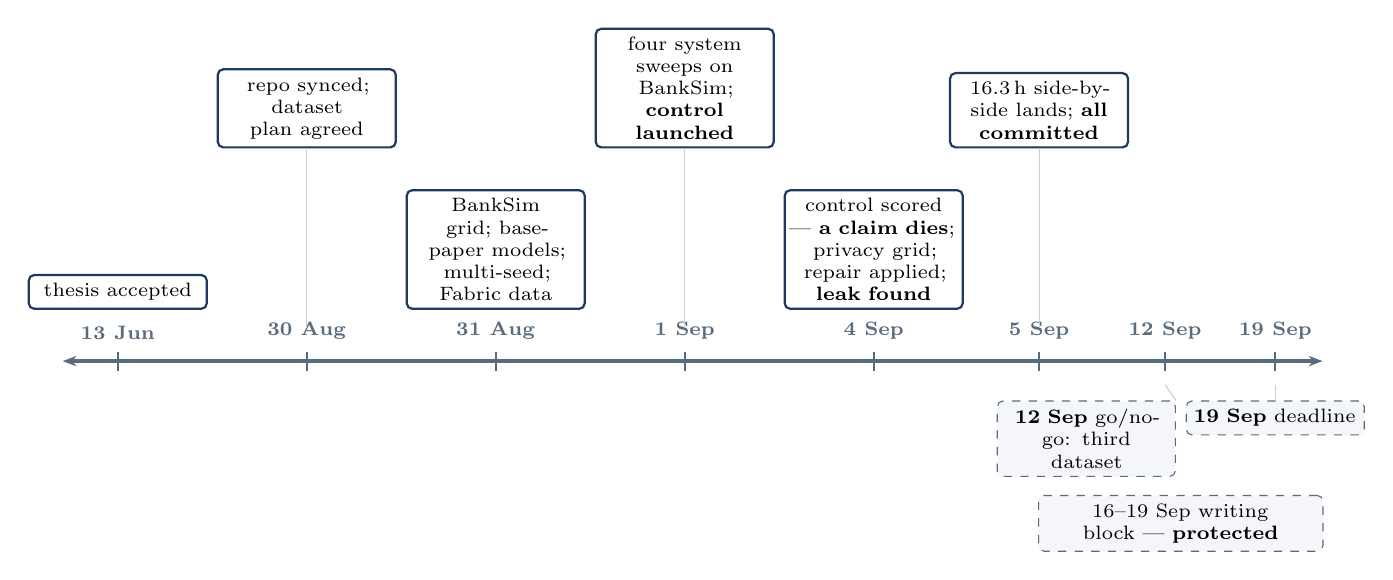
\begin{tikzpicture}[font=\scriptsize,
  ev/.style={draw=navy,fill=white,rounded corners=2pt,inner sep=3pt,align=center,text width=2.05cm,thick},
  fut/.style={draw=steel,dashed,fill=wash,rounded corners=2pt,inner sep=3pt,align=center,text width=2.05cm},
  tick/.style={draw=steel,thick},
  lead/.style={draw=rule,thin}]
  \draw[{Stealth[length=5pt]}-{Stealth[length=5pt]},steel,very thick] (0,0) -- (16,0);
  \foreach \x/\d in {0.7/{13 Jun}, 3.1/{30 Aug}, 5.5/{31 Aug}, 7.9/{1 Sep}, 10.3/{4 Sep}, 12.4/{5 Sep}, 14.0/{12 Sep}, 15.4/{19 Sep}}
    { \draw[tick] (\x,-0.12) -- (\x,0.12); }
  \foreach \x/\d in {0.7/{13 Jun}, 3.1/{30 Aug}, 5.5/{31 Aug}, 7.9/{1 Sep}, 10.3/{4 Sep}, 12.4/{5 Sep}}
    { \node[above=1pt,text=steel] at (\x,0.12) {\textbf{\d}}; }
  \foreach \x/\d in {14.0/{12 Sep}, 15.4/{19 Sep}}
    { \node[above=1pt,text=steel] at (\x,0.12) {\textbf{\d}}; }

  % row A (close to the line)
  \node[ev,above=6.5mm] at (0.7,0) (e1) {thesis accepted};
  \node[ev,above=6.5mm] at (5.5,0) (e3) {BankSim grid; base-paper models; multi-seed; Fabric data};
  \node[ev,above=6.5mm] at (10.3,0) (e5) {control scored --- \textbf{a claim dies}; privacy grid; repair applied; \textbf{leak found}};
  % row B (further out, with leader lines)
  \node[ev,above=27mm] at (3.1,0) (e2) {repo synced; dataset plan agreed};
  \node[ev,above=27mm] at (7.9,0) (e4) {four system sweeps on BankSim; \textbf{control launched}};
  \node[ev,above=27mm] at (12.4,0) (e6) {16.3\,h side-by-side lands; \textbf{all committed}};
  \draw[lead] (3.1,0.42) -- (e2.south); \draw[lead] (7.9,0.42) -- (e4.south);
  \draw[lead] (12.4,0.42) -- (e6.south);

  % future, below the line
  \node[fut,below=5mm] at (13.0,0) (e7) {\textbf{12 Sep} go/no-go: third dataset};
  \node[fut,below=5mm] at (15.4,0) (e8) {\textbf{19 Sep} deadline};
  \node[fut,below=17mm,text width=3.4cm] at (14.2,0) (e9) {16--19 Sep writing block --- \textbf{protected}};
  \draw[lead] (14.0,-0.3) -- (e7.north east); \draw[lead] (15.4,-0.3) -- (e8.north);
\end{tikzpicture}
\caption{The period. Everything above the line has happened and is on disk; everything below it is
planned. The 16--19 September writing block is protected: if the third dataset overruns, the dataset
is cut, not the writing.}
\end{figure}

\subsection{First, close the three loose ends a reviewer would find (31 August)}

Before adding anything new we closed the three defects from Section~\ref{sec:bad} that were cheapest
to fix and most damaging to leave.

\textbf{The MCC contradiction (B3) was resolved, and the resolution was not what the report guessed.}
Thirteen full 30-epoch runs established that training is bitwise deterministic for a fixed triple of
\emph{(seed, torch version, CPU thread count)} --- but two of our scripts were using different thread
counts, so they had never been running the same arithmetic. At seed 42 the tuned configuration scores
0.708 / 0.746 / 0.800 at 4 / 2 / 8 threads, while the hand-set default is bitwise \emph{invariant}. So
the report's ``large batch causes instability'' hypothesis was right about the cause and wrong about
its nature: this is float reduction-order sensitivity, not run-to-run randomness. \textbf{MCC 0.313 is
withdrawn} --- it is not reproducible under any condition we tested. Over five seeds the honest
headline became a distribution: \textbf{tuned 0.753\,$\pm$\,0.055, default 0.706\,$\pm$\,0.076,
difference $+0.047$ at $p=0.34$} --- statistically indistinguishable, and the \emph{default} is the
noisier of the two. The root cause was that \texttt{torch} was listed as optional and unpinned; it is
now pinned at 2.12.0, and \textbf{every reported detector number now requires a stated torch version
and thread count}.

\textbf{The measured Fabric data went into the report (B4)}, replacing the retired 85\,TPS / 180\,ms
with 2115.9\,ms mean latency and the 40.3\,TPS goodput curve. The measurement also exposed a design
mismatch the simulated layer had hidden: the incentive scheme awards a \textbf{+15-token bonus for
latency below 300\,ms}, which is \emph{unreachable} on a 2.1-second Raft floor.

\textbf{And the objective function was de-duplicated:} \texttt{metrics.py} still held a superseded
unbounded formula while the methodology chapter described a bounded one. There is now one definition,
verified bit-identical over 2{,}000 random metric dictionaries.

\subsection{The dataset question --- and the decision to keep ULB}
\label{sec:ulb}

This is the fork the rest of the work hangs on.

\begin{decision}{1 --- Add a second dataset, and \emph{keep} the first one as a live condition}
\qlabel{Question raised:} ULB has no customer identities, so the detector's windows stitch together
unrelated cardholders. That may be the whole reason our temporal architecture lost to a plain CNN
(0.770 vs 0.459 on the original ablation). Do we \textbf{replace} ULB with an entity-linked dataset,
or \textbf{keep} it and run both?

\qlabel{Decision taken:} Keep ULB, add BankSim, and re-run \emph{every} comparison on both under the
same code. BankSim first among the candidates --- one CSV, 594{,}643 transactions, 7{,}200 frauds,
4{,}112 customers with roughly a hundred transactions each, small enough to iterate in minutes.

\qlabel{Why:} Three reasons. (i)~ULB is the dataset the accepted thesis stands on; dropping it would
make every extension result incomparable with the submitted report, and the report would be orphaned.
(ii)~A claim can only be shown to be \emph{dataset-dependent} if both datasets are measured --- a
single new dataset replaces one narrow story with a different narrow story. (iii)~Rule~4: choosing the
dataset on which our architecture looks better, and dropping the one where it does not, is
result-shopping.

\qlabel{Outcome --- and it cut both ways:}
\begin{itemize}[topsep=2pt]
\item \textbf{It paid immediately.} Entity-linked windows help \emph{every} architecture by
$+0.0999$ to $+0.1717$ MCC, so ``temporal complexity does not pay'' was a statement about
entity-\emph{less} windows, not about time. The differential-privacy collapse replicated on the second
dataset --- and its \emph{direction} flipped, which neither dataset shows alone.
\item \textbf{It also produced the two most uncomfortable findings of the period, and both are
ULB-only.} Keeping ULB is the only reason we discovered that the deployed hyperparameter search was
validating on memorised rows (Section~\ref{sec:obj13}), and the only reason we discovered that a ULB
result from 30 August no longer reproduces (Section~\ref{sec:obj17}). Had we dropped ULB, both defects
would still be in the work and neither would be known.
\item \textbf{The honest cost:} two ULB result files are currently not quotable, and one reproduction
failure is recorded as \emph{unexplained}. Keeping ULB bought us the knowledge and the bill together.
\end{itemize}
\end{decision}

\begin{warnbox}{A trap the second dataset nearly set --- caught before it ran}
BankSim's raw CSV emits fraudulent rows \emph{adjacently inside each time step}: 3{,}635 adjacent fraud
pairs in file order versus 84 after shuffling within the step. A \texttt{step} is a whole day, so that
adjacency is an artefact of how the simulator wrote the file, not a property of the world. Had we
windowed in file order, the \emph{global-window control arm} would have shown
$P(\text{fraud}_t \mid \text{fraud}_{t-1}) = 0.50$ --- the control would have looked strongly
predictive and the entire entity-linkage experiment would have been quietly destroyed. With a seeded
within-step tie-break the numbers are global \textbf{0.0117} against a base rate of 0.0121 (no signal,
which correctly reproduces the ULB situation) and customer-linked \textbf{0.3615}. \emph{Any dataset
whose time column is coarser than its row order carries an implicit ordering that is an artefact of
generation.} This check is now mandatory before windowing any new dataset.
\end{warnbox}

\subsection{What the second dataset said about our own detector (31 August)}

With BankSim wired in we re-implemented the base paper's comparison honestly --- all four of its
classifiers and all four of its optimisers, re-run on our data rather than copied from its tables ---
and ran a $2\times 7$ grid (two window types $\times$ seven architectures, three seeds).

\begin{center}\small
\begin{tabularx}{\linewidth}{@{}p{4.6cm} X@{}}
\toprule
\textbf{Result} & \textbf{Reading} \\
\midrule
Entity-linked windows help every architecture, $+0.0999$ to $+0.1717$ MCC & The window was the problem, not the sequence model. The ULB negative result does not generalise. \\
On linked windows ADTCN ranks \textbf{7 of 7} (0.7089), behind its own no-attention ablation DTCN (0.7733) and a plain CNN & \dots but ADTCN is still the wrong sequence model. Best linked: LSTM 0.7805. \\
On ULB global windows ADTCN ranks \textbf{5 of 7} (0.3296); ResNet-1D leads at 0.5995 & Consistent with the above: our detector is a measured component, not a winning one. \\
Attention's contribution \textbf{flips sign} between the two settings: $-0.0645$ on BankSim linked, $+0.0502$ on ULB global & A single-factor ablation (DTCN is deliberately ADTCN-minus-attention) showing the architecture choice is setting-dependent. \\
On ULB, \textbf{all five optimisers hit exactly 5.0000} --- the theoretical ceiling & Not a result about optimisers. This is what opened the surrogate audit in Section~\ref{sec:obj13}. \\
\bottomrule
\end{tabularx}
\end{center}

\begin{keybox}{How we report ADTCN and DB-BOA --- a decision, not an accident}
Neither is a title claim, so neither has to win, but neither may be \emph{described} as winning. They
are reported as \textbf{measured components}: ``we built it, measured it honestly, and it did not beat
the simple baseline'' is a legitimate result in a systems paper. What is not legitimate is quietly
choosing the setting where it looks better. We also state plainly that \textbf{no number from the base
paper is reproduced} --- their results are MATLAB runs on their own data; we re-ran their methods on
ours, and the filter ceiling was cut identically for every optimiser to fit a CPU budget.
\end{keybox}

\subsection{Taking the system claims off one dataset (1 September)}

The expansion had reached the detector and stopped. Four of the six title claims were still backed by
ULB alone --- not by choice, but because four sweep scripts hard-coded the ULB loader (B2).

\begin{decision}{2 --- Breadth across \emph{claims} before breadth across \emph{datasets}}
\qlabel{Question raised:} With one new dataset working, do we add a \emph{third} dataset (which sounds
more thorough), or spend the time getting the \emph{existing} claims off ULB?

\qlabel{Decision taken:} Get every claim off ULB once, before any claim goes to a third dataset.

\qlabel{Why:} A claim tested on three datasets while four sibling claims sit on one is a lopsided
table, and a reviewer attacks the four, not the one. This is now Rule~8.

\qlabel{Outcome:} A shared dataset-resolution module, all four sweeps taking
\texttt{--dataset}/\texttt{--partition}, provenance stamped into every result file, and four sweeps
re-run on BankSim in 3\,h\,15\,m. \textbf{Five of six title claims came off ULB}; the sixth group is
dataset-independent by design. Two latent bugs surfaced in the smoke test that would have spoiled the
overnight run --- and two \emph{worse} ones surfaced by reading the output instead of trusting the exit
code: the run was overwriting the original ULB figures in place, and the generated prose asserted ULB
conclusions regardless of what had been measured. A draft that contradicts the table printed directly
above it is the B9 failure with the numbers left in. \textbf{Regenerating any draft now takes seconds
and reads from the data.}
\end{decision}

\subsection{The control that killed our best new claim (1--4 September)}
\label{sec:control}

The BankSim sweeps produced a striking finding: Krum, which rejects poisoned weight vectors perfectly,
appeared to \emph{pay} 1.5--12.6 percentage points of accuracy for that protection when organisations
hold disjoint customers. We had a mechanism for it, and it was the most quotable thing in the objective.

It was also confounded. Every BankSim-vs-ULB comparison had changed \textbf{two things at once}: the
dataset \emph{and} the way organisations were partitioned.

\begin{figure}[h]
\centering
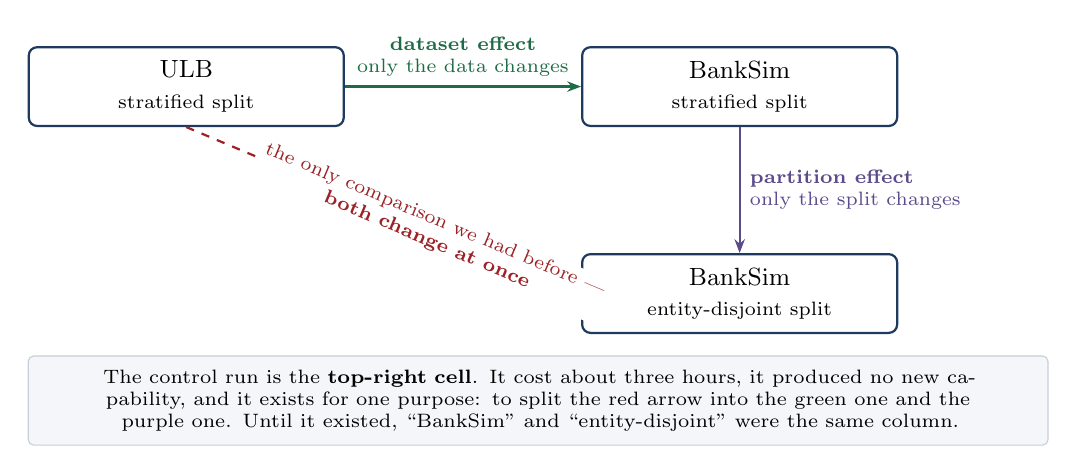
\begin{tikzpicture}[font=\small,
  cell/.style={draw=navy,fill=white,rounded corners=3pt,minimum width=4.0cm,minimum height=1.0cm,align=center,thick},
  ar/.style={-{Stealth[length=5pt]},thick}]
\node[cell] (a) {ULB\\\scriptsize stratified split};
\node[cell,right=3.0cm of a] (b) {BankSim\\\scriptsize stratified split};
\node[cell,below=1.6cm of b] (c) {BankSim\\\scriptsize entity-disjoint split};
\draw[ar,okgreen] (a) -- node[above,font=\scriptsize,text=okgreen,align=center]{\textbf{dataset effect}\\\scriptsize only the data changes} (b);
\draw[ar,lilac] (b) -- node[right,font=\scriptsize,text=lilac,align=left]{\textbf{partition effect}\\\scriptsize only the split changes} (c);
\draw[ar,badred,dashed] (a.south) -- node[sloped,font=\scriptsize,text=badred,align=center,pos=0.62,fill=white,inner sep=1.5pt]{the only comparison we had before ---\\\textbf{both change at once}} (c.west);
\node[draw=rule,fill=wash,rounded corners=2pt,anchor=north west,text width=12.6cm,align=center,font=\scriptsize,inner sep=5pt]
 at ($(a.south west)+(0,-2.9)$)
 {The control run is the \textbf{top-right cell}. It cost about three hours, it produced no new capability, and it exists for one purpose: to split the red arrow into the green one and the purple one. Until it existed, ``BankSim'' and ``entity-disjoint'' were the same column.};
\end{tikzpicture}
\caption{Why the confound control had to exist. Without the top-right cell, ``BankSim'' and
``entity-disjoint'' are the same column and no divergence can be attributed to either.}
\end{figure}

\begin{decision}{3 --- Run a three-hour control instead of starting the third dataset}
\qlabel{Question raised:} We have a strong new finding and a deadline. Do we build on it (third
dataset), or spend three hours trying to break it?

\qlabel{Decision taken:} Run the control first --- BankSim with a \emph{stratified} split, so the
dataset changes without the partition changing.

\qlabel{Why:} If the finding is wrong, everything built on top of it inherits the error, and a third
dataset would have added a third \emph{confounded} column at the same time.

\qlabel{Outcome --- the control falsified our own claim.} Krum is negative in \textbf{7 of 8 cells
under the stratified partition too}, where organisations are \emph{not} customer-disjoint. The dataset
effect is negative in all 8 rows ($-1.06$ to $-17.27$\,pp); the partition effect changes sign --- and at
$n=7$ it is \textbf{positive in all four rows}, the exact opposite of our stated mechanism.
\textbf{``Krum pays utility under entity-disjointness'' is withdrawn.} Two further pre-registrations
died the same way: lone-attacker isolation also tracks the dataset (it fires 3/3 on \emph{both} BankSim
partitions and 0/3 on ULB), and Monte-Carlo rank fidelity moves $+0.783$ on the dataset axis against
$-0.322$ on the partition axis. \textbf{Every divergence we had attributed to federation structure was
actually BankSim.}
\end{decision}

\begin{center}\small
\begin{tabularx}{\linewidth}{@{}X r r r r r@{}}
\toprule
\textbf{Krum $-$ FedAvg (pp, balanced acc.)} & \textbf{ULB/strat} & \textbf{BS/strat} & \textbf{BS/entity} & \textbf{dataset} & \textbf{partition} \\
\midrule
$n{=}5$ sign-flip & $+0.03$ & $-4.62$ & $-11.20$ & $-4.65$ & $-6.58$ \\
$n{=}5$ scaled & $+12.49$ & $+0.54$ & $-1.48$ & $-11.95$ & $-2.03$ \\
$n{=}5$ gaussian & $-0.01$ & $-1.07$ & $-12.57$ & $-1.06$ & $-11.50$ \\
$n{=}5$ label-flip & $+0.04$ & $-5.50$ & $-11.13$ & $-5.54$ & $-5.63$ \\
$n{=}7$ sign-flip & $+0.13$ & $-9.15$ & $-4.73$ & $-9.28$ & \textbf{$+4.43$} \\
$n{=}7$ scaled & $+12.48$ & $-4.79$ & $-1.65$ & $-17.27$ & \textbf{$+3.14$} \\
$n{=}7$ gaussian & $+0.00$ & $-11.96$ & $-10.60$ & $-11.96$ & \textbf{$+1.36$} \\
$n{=}7$ label-flip & $+0.00$ & $-11.61$ & $-6.32$ & $-11.61$ & \textbf{$+5.28$} \\
\bottomrule
\end{tabularx}
\end{center}

\textbf{What survives, and it is worth keeping:} Krum rejects the attacker \textbf{8 out of 8 in all
three conditions} --- the security property replicates and is now three-condition solid. Krum
\emph{can} cost utility, by an amount that tracks the dataset. \textbf{No mechanism for that cost is
currently on record, and saying so is the honest position.} An unexplained measured effect is a
result; a mechanism invented to cover it is not.

\begin{warnbox}{A metric artefact we then had to map, cell by cell}
In several runs the \emph{attacked} FedAvg model scores \emph{above} its own no-attack reference. An
attack cannot genuinely improve a model --- this is balanced accuracy rewarding noise that pushes the
decision boundary toward the positive class. The contamination is condition-graded: \textbf{0 of 8
(ULB), 2 of 8 (BankSim/stratified), 5 of 8 (BankSim/entity-disjoint)} --- i.e.\ worst precisely in the
condition we had headlined, and \emph{every} cell worse than $-5$\,pp there is a contaminated one. On
the clean cells only, the entity-disjoint cost is $-4.73$ to $-1.48$\,pp, not $-12.57$ to $-1.48$.
Crucially, on the three cells that are clean in \emph{all three} conditions the withdrawal reproduces
--- so it survives the filter rather than being produced by it.
\end{warnbox}

\subsection{Propagating a withdrawal is its own job (4 September)}

A claim is not withdrawn when you decide it is wrong. It is withdrawn when it is out of the generators.

A repository-wide sweep found the dead mechanism alive in \textbf{two script-generated drafts} and the
supervisor brief carrying a separate over-claim. All were fixed \emph{at the generator} and
regenerated. The sweep also exposed a class of bug worth naming: the offending sentence was emitted by
a \textbf{single-run} generator --- a script that reads one result file \emph{structurally cannot} see a
dataset-versus-partition effect, so any attribution it prints is unfalsifiable by its own evidence.
\textbf{A generator may only assert what its own input can falsify.} Attribution now lives only in the
collator that reads all three conditions.

One incidental discovery: the supervisor brief's PDF had been silently stuck two revisions behind its
source for days, because the LaTeX installation was missing scalable Type\,1 fonts and
\texttt{microtype}'s auto-expansion was aborting every build. \textbf{The document the supervisor
actually reads had not been rebuilt, and nobody would have seen it.} Fixed.

\subsection{The privacy budget: we measured it, and then retired it}
\label{sec:obj17}

The censored statistic from B7 was the cheapest thing on the board to fix, and it was the only open item
that could \emph{un-withdraw} a claim. \epsst{} is defined as the largest privacy budget at which
rewards are still mis-ranked; the weight channel was still failing at $\eps=3000$, the top of the grid,
so every improvement factor we quoted was a lower bound.

\begin{decision}{4 --- Extend the grid \emph{and} the draw count, on one shared grid for all three conditions}
\qlabel{Question raised:} Extend the grid (test further out) or raise the repeat count (measure the
rate more precisely)? They fix different things.

\qlabel{Decision taken:} Both, and \textbf{every condition re-run on the same extended grid} --- 11
points out to $\eps=30000$, then a second pass at 1000 draws on the budgets that actually decide each
threshold. Full scope approved, about 4 hours of CPU.

\qlabel{Why:} Three columns on three different grids are not comparable. And a correction found
\emph{before} the run showed the two knobs are not interchangeable: more budgets test further out;
more draws tighten the estimate at a fixed budget.

\qlabel{Outcome:} The stated goal was met --- \textbf{all three conditions de-censored}, every factor
became a measurement rather than a lower bound. \textbf{And then the measurement turned out to be the
wrong thing to quote.}
\end{decision}

\begin{keybox}{The correction that reframed the whole objective --- and it came from reading code, not from a result}
$\epsst = \max\{\eps : \text{inversion rate} > 0\}$ is \textbf{monotone non-decreasing in both the draw
count and the grid extent}. The random draws are seeded by repeat index, so a 1000-draw run strictly
\emph{contains} the 100-draw run; and a longer grid can only add candidates to a maximum.
\textbf{Neither knob can ever lower \epsst.} So ``de-censoring'' never means a population quantity was
located --- it means the budgets we added happened to show no failures. \epsst{} is properly read as
\emph{``the largest budget at which a failure was caught''}, and it gets worse the harder anyone looks.
That is a property of the estimator, not of the mechanism.
\end{keybox}

The two passes then demonstrated exactly that, twice in one day. After the grid pass,
BankSim/entity-disjoint was the \emph{best}-supported column and we wrote that it should be preferred
over ULB. Six hours later, looking $10\times$ harder found one failure in a thousand at the top of its
probe grid --- its threshold rose, its factor rose from $33\times$ to $\ge 100\times$, and \textbf{it
became a lower bound again}. The trustworthiness ordering flipped back.

\begin{center}\small
\begin{tabularx}{\linewidth}{@{}X c c c@{}}
\toprule
\textbf{The same data, read at three different rate thresholds} & \textbf{rate $>0$} & \textbf{rate $>0.01$} & \textbf{rate $>0.05$} \\
\midrule
ULB / stratified & $60\times$ & $20\times$ & $33\times$ \\
BankSim / stratified & $30\times$ & $60\times$ & $20\times$ \\
BankSim / entity-disjoint & $\ge100\times$ & $33\times$ & $33\times$ \\
\bottomrule
\end{tabularx}\\[3pt]
{\footnotesize The factor swings from $20\times$ to $\ge100\times$ on an arbitrary cut-off,
\textbf{and the ranking of the three conditions changes with it.} Only the leftmost column was ever
published.}
\end{center}

\begin{decision}{5 --- Retire the improvement factor as a headline}
\qlabel{Question raised:} We finally have measured numbers. Do we publish the factor?

\qlabel{Decision taken:} No. \textbf{Retire it}, and carry the contribution on two threshold-free
statements instead.

\qlabel{Why:} Rule~4. Picking whichever cut-off flatters the mechanism is result-shopping, and no
single number from this family is defensible. The mechanism does not need it.

\qlabel{Outcome --- what carries the claim now:}
\begin{enumerate}[topsep=2pt,label=(\arabic*)]
\item \textbf{The ordering.} The output channel mis-ranks rewards no more often than the weight
channel --- 12 of 12 probed budgets, and 11/11, 11/11, 10/11 across the full grid. It is \emph{paired
within each draw}, so sample size changes its precision, never its direction. It has now survived
three conditions, two sample sizes and two metrics.
\item \textbf{The rank-fidelity gap at a stated budget}, which needs no threshold at all. At
$\eps=50$: $\rh = -0.199 \rightarrow +0.995$ (ULB), $+0.017 \rightarrow +0.945$ (BankSim/stratified),
$-0.070 \rightarrow +0.805$ (BankSim/entity-disjoint). Same direction in all three.
\end{enumerate}
And one genuinely reassuring result: the four fragile thresholds that had rested on a single inverted
draw out of 100 became 7, 11, 16 and 10 per 1000 --- all consistent with a true rate near 0.01.
\textbf{The fragility was about precision, never about existence.}
\end{decision}

\begin{figure}[h]
\centering
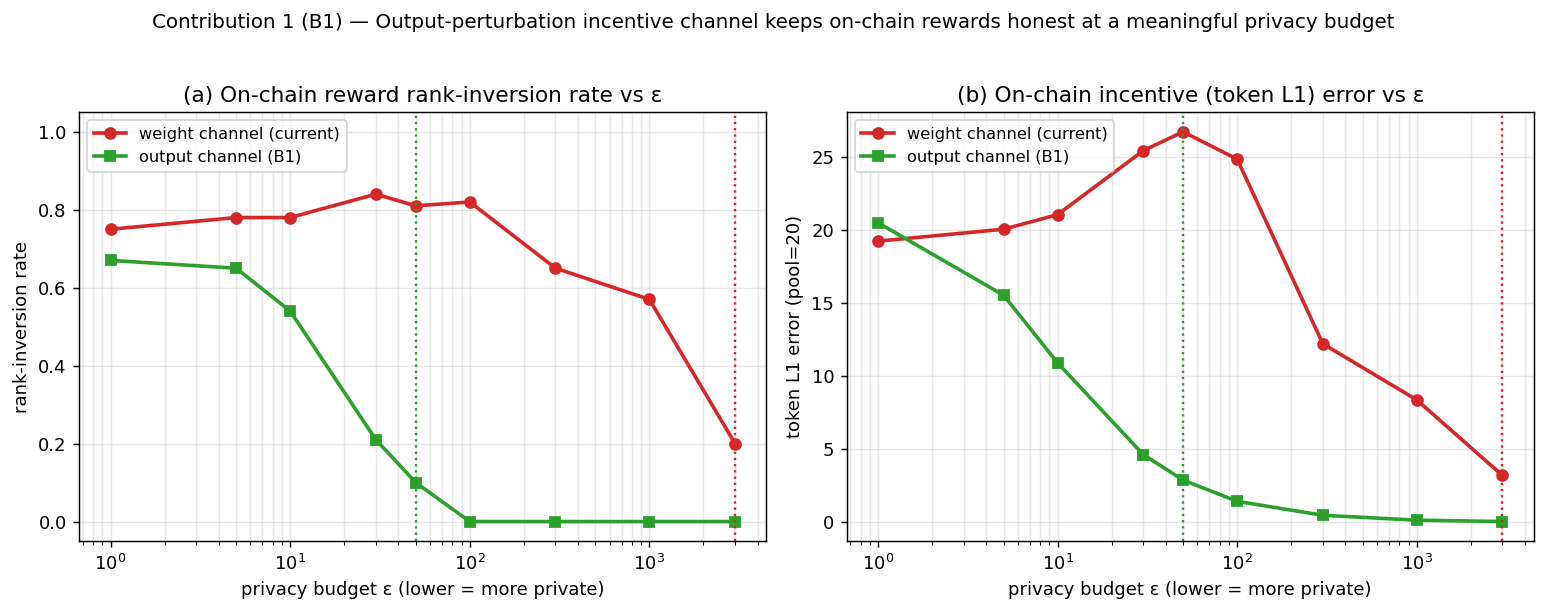
\includegraphics[width=\linewidth]{db_boa_framework/results/private_incentive_channel.png}
\caption{The contribution, on the extended 11-point grid. \textbf{(a)} How often the on-chain reward
ranking is wrong, against the privacy budget; \textbf{(b)} the resulting token error. The green
(output) channel reaches faithful rewards roughly an order of magnitude earlier in $\eps$ than the red
(weight) channel. \textbf{It is the separation between the curves that is the claim, not the ratio of
the two dotted lines} --- Section~\ref{sec:obj17} explains why the ratio is not a stable statistic.}
\end{figure}

\begin{warnbox}{The cost nobody was auditing: a ULB result no longer reproduces}
While verifying that the longer run contained the shorter one, we re-ran the nine historical budgets at
identical seeds. \textbf{Both BankSim conditions reproduced 9 of 9 bitwise. ULB moved in 13 of 18
cells}, and its ground-truth contribution split moved with them. ULB \emph{does} reproduce itself
same-day (11 of 11), so it is deterministic under fixed conditions --- the 30 August divergence is a
change of \emph{conditions}. We then eliminated everything reachable: every code change on the ULB path
was audited and shown provably inert for ULB; every configuration dictionary was compared
literal-by-literal; thread-count sensitivity was tested directly (all six weight tensors bit-identical).
What remains is the torch/numpy version at the time --- \textbf{and that is unrecoverable, because no
stored result recorded the stack it ran under.}

\textbf{We recorded it as unexplained rather than guessing a cause.} The durable fix shipped the same
day: torch version, thread count, numpy version, Python version and platform are now written into
\emph{every} sweep result file. \emph{That diagnosis took a day and produced no number; the guard is
what stops the next one costing the same.}
\end{warnbox}

\subsection{The search the framework is named after (4--5 September)}
\label{sec:obj13}

The last and largest piece of work in the period. It started from B5 --- five different optimisers
reporting exactly 5.0000 on ULB --- and it ended somewhere considerably worse than we expected.

\subsubsection*{The diagnosis} DB-BOA searches for the detector's hyperparameters by scoring candidate
configurations on a small surrogate model. That scoring function \textbf{re-drew its own train/validation
split and its own random seed on every call}, which makes it a \emph{random function of its input}. Three
measurements followed:

\begin{itemize}
  \item A \textbf{fixed} configuration re-evaluated 25 times on ULB spans 3.4497--5.0000 and touches
  the theoretical ceiling \emph{once, with no search involved}.
  \item Changing which rows are sampled moves the score about as much as changing the model does
  (between-seed spread 1.0471 against a configuration-to-configuration range of 1.0794).
  \item \textbf{One of the two search axes was arithmetically dead.} A batch-size floor,
  \texttt{max(32, 1400 // spe)}, evaluated to 32 for \emph{every} value of \texttt{steps\_per\_epoch} in
  the searched range. The advertised two-dimensional search was one-dimensional, and every reported
  \texttt{steps\_per\_epoch} optimum was arbitrary.
\end{itemize}

\textbf{This strengthens the negative result rather than softening it}: a search that cannot rank its
candidates returns an essentially arbitrary one, so tying a sensible hand-set default is the
\emph{expected} outcome.

\subsubsection*{Then the shipped path was checked, and it was worse}

\begin{warnbox}{The audit had never measured the pipeline that ships}
The diagnostic script built its surrogate from a 6{,}000-row pool. The \emph{deployed} pipeline uses a
different function that returns \textbf{3{,}000 rows}. At ULB's 0.173\% fraud rate, that pool holds
\textbf{5 unique fraud transactions} --- against a minimum of 30 the surrogate demands. So it drew 30
``fraud rows'' \emph{with replacement}: 5 transactions repeated about six times each. After the 70/30
split, \textbf{9 of 9 validation positives were copies of rows in the training half}.

\textbf{The 5.0000 ceiling was memorisation, not luck on nine rare rows.} And the repair we had spent
three days designing did \emph{not} close it: stratifying the split guarantees positives on both sides,
which with five unique transactions is precisely how copies land on both sides. BankSim was clean
throughout (38 and 75 unique frauds). \textbf{Diagnostics must run on the path that ships.}
\end{warnbox}

\begin{figure}[h]
\centering
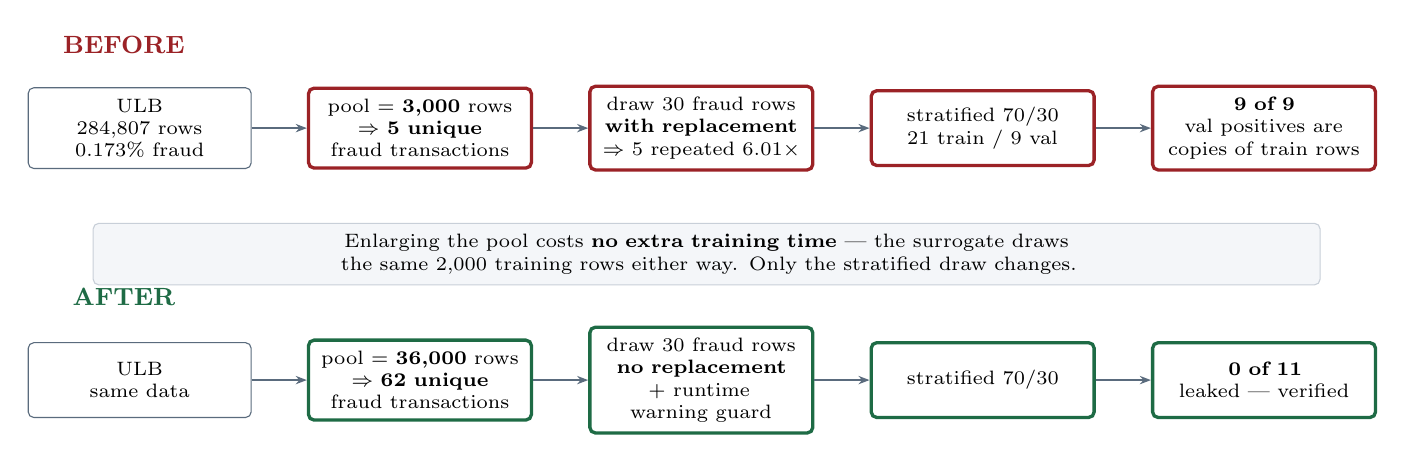
\begin{tikzpicture}[font=\scriptsize,
  bx/.style={draw=steel,fill=white,rounded corners=2pt,align=center,inner sep=4pt,text width=2.55cm,minimum height=0.95cm},
  bad/.style={bx,draw=badred,very thick},
  good/.style={bx,draw=okgreen,very thick},
  ar/.style={-{Stealth[length=4pt]},draw=steel,thick}]

\node[font=\bfseries\small,text=badred] at (-0.2,1.05) {BEFORE};
\node[bx] (p1) at (0,0) {ULB\\284{,}807 rows\\0.173\% fraud};
\node[bad,right=7mm of p1] (p2) {pool = \textbf{3{,}000} rows\\$\Rightarrow$ \textbf{5 unique}\\fraud transactions};
\node[bad,right=7mm of p2] (p3) {draw 30 fraud rows\\\textbf{with replacement}\\$\Rightarrow$ 5 repeated $6.01\times$};
\node[bad,right=7mm of p3] (p4) {stratified 70/30\\21 train / 9 val};
\node[bad,right=7mm of p4] (p5) {\textbf{9 of 9}\\val positives are\\copies of train rows};
\draw[ar](p1)--(p2); \draw[ar](p2)--(p3); \draw[ar](p3)--(p4); \draw[ar](p4)--(p5);

\node[font=\bfseries\small,text=okgreen] at (-0.2,-2.15) {AFTER};
\node[bx] (q1) at (0,-3.2) {ULB\\same data};
\node[good,right=7mm of q1] (q2) {pool = \textbf{36{,}000} rows\\$\Rightarrow$ \textbf{62 unique}\\fraud transactions};
\node[good,right=7mm of q2] (q3) {draw 30 fraud rows\\\textbf{no replacement}\\+ runtime warning guard};
\node[good,right=7mm of q3] (q4) {stratified 70/30};
\node[good,right=7mm of q4] (q5) {\textbf{0 of 11}\\leaked --- verified};
\draw[ar](q1)--(q2); \draw[ar](q2)--(q3); \draw[ar](q3)--(q4); \draw[ar](q4)--(q5);

\node[draw=rule,fill=wash,rounded corners=2pt,inner sep=4pt,text width=15.3cm,align=center] at (7.2,-1.6)
 {Enlarging the pool costs \textbf{no extra training time} --- the surrogate draws the same 2{,}000 training rows either way. Only the stratified draw changes.};
\end{tikzpicture}
\caption{The leak, and the fix. The defect was in the \emph{pool}, one layer below where the planned
repair operated, which is why the repair could not reach it.}
\end{figure}

\begin{decision}{6 --- Fix the pool by enlarging it, not by re-weighting or clamping}
\qlabel{Question raised:} Three ways to stop the surrogate validating on memorised rows. (a)~Enlarge the
pool so 30 genuinely distinct fraud rows exist at the real rate. (b)~Oversample fraud \emph{into} the
pool. (c)~Never sample with replacement --- accept whatever few unique frauds exist.

\qlabel{Decision taken:} (a). Pool raised from 3{,}000 to 36{,}000 rows for both datasets, plus a
runtime warning that fires if the replacement branch is ever taken again.

\qlabel{Why:} (b) would make the surrogate see a fraud rate that is not the dataset's --- the exact
defect the function was written to avoid. (c) would leave ULB's surrogate training on \textbf{five}
fraud rows, which is honest and useless. Only (a) keeps the rate real \emph{and} the positives distinct.
The warning was added because \textbf{the cost of this defect was its silence}: a config value alone
would fix today's datasets and let the next one reintroduce it without a sound.

\qlabel{Outcome:} Verified 0 of 11 validation positives leaked, on both datasets, in both modes.
\end{decision}

\subsubsection*{The repair, and three defects it would have shipped with}

Applying a patch to the scoring function turned up three ways it would have quietly corrupted its own
evidence, all found by checking rather than trusting:

\begin{enumerate}
  \item The patch \textbf{silently re-pointed the diagnostic script} --- the one that produced this
  entire objective's evidence base --- at the new default mode. It would have reported a within-seed
  standard deviation of \textbf{exactly 0.0000} and read as \emph{``the objective was always fine''},
  which is the precise opposite of the finding. It now pins the old behaviour explicitly, with the
  reason written at every call site so it is not ``simplified'' away later.
  \item The same silent switch in the base-paper comparison script, whose stored results \emph{are} the
  5.0000 evidence. It now stamps the mode into its own output and \textbf{refuses to overwrite} a file
  recorded under a different one. A warning would not do --- a warning scrolls off the top of a six-hour run.
  \item A pre-existing filename collision in which two separate result tracks overwrote each other,
  leaving only whichever ran last. \textbf{This was the third instance of the same class of bug} in a
  fortnight: an artefact whose only copy lives somewhere the next run can destroy.
\end{enumerate}

We also verified the old behaviour is reproduced \textbf{bit-for-bit} --- three configurations agreeing
to ten decimal places against a saved copy of the pre-patch module --- so the comparison runs against a
live baseline rather than a remembered one.

\begin{decision}{7 --- Run the comparison at full deployment budget, against the recommendation}
\qlabel{Question raised:} The side-by-side could run cheaply (about 1.1\,h, matched to the base-paper
budget) or at the \emph{deployed} search budget (about 16.7\,h). The written recommendation was the
cheap option.

\qlabel{Decision taken:} \textbf{The expensive one} --- population $20\times30$, three surrogate
protocols $\times$ three seeds, BankSim only, run detached overnight.

\qlabel{Why:} Only the deployed budget yields configurations comparable to the one actually shipped in
our results (142 filters / 76 steps-per-epoch). A cheaper run would have answered a question we were not
asking. BankSim only, because at that moment ULB's pool did not describe its own deployment, so a ULB arm
would have cost 17 hours to produce a number needing a caveat longer than the result.

\qlabel{Outcome:} 16.3 hours, 9 of 9 searches completed, clean exit. \textbf{Not one of the nine
searched configurations beats a hand-set 128 filters / 150 steps-per-epoch.} If this run ever has to be
repeated, repeat it at the same budget --- do not ``optimise'' it back down.
\end{decision}

\begin{center}\small
\begin{tabularx}{\linewidth}{@{}l c r c X@{}}
\toprule
\textbf{Surrogate mode} & \textbf{Filters chosen} & \textbf{paired \dl{} vs default} & \textbf{wins/7} & \textbf{Reading} \\
\midrule
\texttt{legacy} (unrepaired) & 81 / 69 / 135 & $-0.2027$ / $-0.1130$ / $-0.1780$ & 0 / 1 / 1 & every seed below the default \\
\texttt{deterministic} & 137 / 56 / 62 & $-0.1654$ / $-0.1647$ / $\mathbf{-0.0720}$ & 0 / 2 / \textbf{4} & holds the best single search \\
\texttt{averaged} (shared draws) & 137 / 146 / 149 & $-0.1654$ / $-0.3512$ / $-0.3716$ & 0 / 1 / 1 & converges, and generalises worst \\
\midrule
\emph{the configuration we shipped} & 142 filters, 76 spe & $-0.1900$ & 2 & also loses to the default \\
\bottomrule
\end{tabularx}\\[3pt]
{\footnotesize Objective seeds are 42 / 7 / 123 in every row. Mean paired difference across all nine:
$\mathbf{-0.1982}$. Compared \textbf{paired} on seven shared held-out draws, because the yardstick uses
common random numbers --- judging these by the $\pm 0.4$ spreads on the individual means would call a
real difference ``noise''.}
\end{center}

\subsubsection*{Two findings that inverted what we had predicted}

\begin{keybox}{1. Common random numbers, not determinism, is what makes a noisy search reproducible}
We predicted the chosen configuration would keep scattering across seeds in \emph{every} mode. The
spread of chosen filter counts: \texttt{legacy} \textbf{66}, \texttt{deterministic} \textbf{81 ---
wider than legacy}, \texttt{averaged} \textbf{12} (on a 5--255 range). \textbf{Freezing the random draw
does nothing; sharing the same draws across candidates is what converges the search.} That design
detail was added almost as an implementation convenience and is empirically the half of the repair that
does the work. This is the most transferable finding of the period and it applies to any noisy
optimisation.
\end{keybox}

\begin{keybox}{2. The mode that converges generalises \emph{worst} --- the noise was accidental regularisation}
On held-out draws: \texttt{deterministic} 3.5857 $>$ \texttt{legacy} 3.5552 $>$ \texttt{averaged}
\textbf{3.4237}. The converged mode is the worst, because with only three shared draws a search that can
finally rank reliably will exploit \emph{those three draws} --- and it converges onto high-filter
configurations (137, 146, 149) that overfit them. \textbf{Making the objective rankable made the search
better at overfitting it.} Both halves of that sentence are measured, and neither is a reason to prefer
the broken objective.
\end{keybox}

\subsubsection*{And one defect the repair itself revealed}

The repair only touched the \emph{surrogate}. The final deployed model still uses the old floored
formula --- but at roughly 400{,}000 training rows that floor never binds, \textbf{so the final model's
second axis was always live and only the surrogate's was dead}. The search was therefore blind to a
dimension the deployed model genuinely responds to. That is worse than ``one axis was wasted'', and the
decision on whether to change it is deliberately still open, because changing it invalidates every
trained model.

\begin{keybox}{The verdict, and why it is the right outcome}
\textbf{The repair works, changes which configuration the search picks, and still does not beat a
hand-set default.} Rule~3 governs: this was \emph{diagnosis of a negative result, not a rescue attempt},
and it was pre-registered as such before any repaired run. The claim ``DB-BOA buys no measured accuracy
gain over the hand-tuned default'' no longer rests on a statistical tie at $p=0.34$ --- it rests on a
direct paired measurement, under three surrogate protocols, at three seeds, at the deployed budget.
\textbf{The negative result got stronger by being attacked.}
\end{keybox}

% =====================================================================
\section{The decision log}

Every fork in the period, with what it produced. This is the part to read if you read nothing else.

{\footnotesize
\renewcommand{\arraystretch}{1.22}
\begin{xltabular}{\linewidth}{@{}p{0.35cm} >{\raggedright\arraybackslash}p{3.1cm} >{\raggedright\arraybackslash}p{4.4cm} X@{}}
\toprule
& \textbf{Question} & \textbf{Answer chosen, and why} & \textbf{What it produced} \\
\midrule
\endfirsthead
\toprule
& \textbf{Question} & \textbf{Answer chosen, and why} & \textbf{What it produced} \\
\midrule
\endhead
1 & Replace ULB with an entity-linked dataset, or keep both? & \textbf{Keep ULB, add BankSim.} A claim is only shown dataset-dependent if both are measured; dropping the losing dataset is result-shopping. & Entity-linkage priced at $+0.10$ to $+0.17$ MCC; DP collapse replicated with a \emph{flipped direction}; \textbf{and} it exposed two ULB-only defects (the memorised-rows leak, the reproduction failure) that would otherwise still be hidden. \\
2 & Third dataset, or get existing claims off ULB? & \textbf{Claims first} (Rule 8). A lopsided table is not rigour. & Five of six title claims off ULB in 3\,h\,15\,m; generic plumbing so a third dataset is loader work only. \\
3 & Build on the new Krum finding, or spend 3\,h trying to break it? & \textbf{Break it.} A control that can overturn a finding outranks a dataset that can add one (now Rule 12). & \textbf{Our best new claim died}, along with two others --- all three were attributions to federation structure that belonged to the dataset. Caught by us, not by a reviewer. \\
4 & Extend the privacy grid, raise the draw count, or both? & \textbf{Both, on one shared grid.} They fix different things and three columns on three grids are not comparable. & All three conditions de-censored; the four fragile thresholds shown to be real; and the estimator shown to be unstable. \\
5 & We finally have measured factors --- publish them? & \textbf{No, retire the factor.} It swings $20\times$ to $\ge100\times$ on an arbitrary cut-off and the ranking changes with it. & The contribution now rests on two threshold-free statements: the ordering (paired, 12/12) and the rank-fidelity gap at a stated budget. \\
6 & Fix the surrogate pool by enlarging, re-weighting, or clamping? & \textbf{Enlarge} (3{,}000 $\to$ 36{,}000) plus a runtime guard. Only this keeps the fraud rate real \emph{and} the positives distinct. & 0 of 11 leaked, verified; and it costs no extra training time. \\
7 & Cheap 1.1\,h comparison or the 16.7\,h deployment budget? & \textbf{The expensive one}, against the written recommendation --- only it yields configurations comparable to what we shipped. & 16.3\,h, 9/9 clean, \textbf{0 of 9 beat the hand-set default}; two predictions inverted; the negative result strengthened. \\
8 & Repair the dead search axis, or drop it? & \textbf{Repair it.} If it turns out not to matter once genuinely alive, that is a \emph{measured} finding; dropping it now asserts the same conclusion without evidence. & The axis is alive but coarse (23 distinct batch sizes across 201 values), and repairing it revealed the deployed model's axis was never dead --- only the surrogate's. \\
9 & The 30 August ULB result does not reproduce. Name a cause? & \textbf{Record it as unexplained.} Guessing the torch version would be inventing a cause. & Two ULB files marked not-quotable, and environment stamping now shipped in every sweep result file. \\
10 & Consolidate or expand, with 15 days left? & \textbf{Consolidate first}, then expand; writing block protected. & The surrogate repair had to precede any third dataset, or that dataset's search arm would be generated on a search we already knew was broken --- and paid for twice. \\
11 & Commit the extension, or keep iterating? & \textbf{Commit.} About 20\,h of results existed only as untracked files. & Two commits on a branch; and a \texttt{.gitignore} rule written for LaTeX was found to be silently swallowing \emph{experiment run logs}. \\
\bottomrule
\end{xltabular}}

% =====================================================================
\section{Where the six claims stand now}

\begin{center}\small
\renewcommand{\arraystretch}{1.2}
\begin{tabularx}{\linewidth}{@{}p{3.1cm} p{2.6cm} X@{}}
\toprule
\textbf{Title claim} & \textbf{Datasets} & \textbf{Status after the period} \\
\midrule
\textbf{Secure} (privacy) & ULB + BankSim $\times2$ splits & \textbf{Replicates, and the second dataset added a new finding.} The DP model collapses to MCC $\approx 0$ everywhere --- but the \emph{direction} differs: on ULB it goes all-negative and accuracy moves only $-0.11$\,pp (it looks almost unharmed while being useless); on BankSim it goes all-positive with 119{,}784 false positives and accuracy $-97.55$\,pp. \emph{An accuracy-reported DP pipeline on 0.17\%-fraud data hides the failure completely} --- an argument for our metric choice, not just for the privacy claim. \\
\textbf{Secure} (Byzantine) & ULB + BankSim $\times2$ & \textbf{Rejection replicates 8/8 in all three conditions.} Krum can cost utility, by an amount that tracks the \textbf{dataset}; the entity-disjointness mechanism is \textbf{withdrawn} and no mechanism is currently on record. \\
\textbf{Incentivized} (collusion) & ULB + BankSim $\times2$ & \textbf{Replicates three times}: 2-of-3 collusion caught, $+40.78/+44.39/+47.40$ (always-fraud) and $+79.52/+86.95/+89.73$ (label-flip). The lone-attacker story \emph{changed}: isolation now fires 3/3 on BankSim (0/3 on ULB) but improves accuracy on \textbf{0 of 3 in every condition} --- the layer fires and does not help. That negative is now three-condition solid. \\
\textbf{Incentivized} (privacy $\leftrightarrow$ incentive) & ULB + BankSim $\times2$ & \textbf{The ordering holds everywhere} (12/12 probed budgets; 11/11, 11/11, 10/11 on the full grid, with one counter-example at $\eps=1$ where \emph{both} channels fail near-totally). The improvement factor is \textbf{retired as a headline}; the $\rh$-gap at a stated budget carries it instead. \\
\textbf{Scalable} (attribution) & ULB + BankSim $\times2$ & Exact-Shapley cost replicates and is \textbf{structural} (113.5 / 140.3 / 120.6\,s at $n{=}12$ over the same 4{,}095 coalitions) --- confirmed and expected, not news. \textbf{``MC top-1 fails from $n\!\approx\!6$'' is withdrawn}: it is intermittent (5/10, 5/10, 3/10) with no consistent pattern. The Monte-Carlo estimator is barely a speed-up below $n\!\approx\!10$ and on ULB at $n{=}5$ it is \emph{slower} than exact. \\
\textbf{RL / Consensus / Blockchain} & dataset-independent & Gini 0.90 $\to$ 0.782 over 5 seeds; degraded-node election 100\% $\to$ 15.2\%; Fabric 2115.9\,ms mean latency, 40.3\,TPS at concurrency 10 with an MVCC knee immediately after. \\
\bottomrule
\end{tabularx}
\end{center}

\begin{figure}[h]
\centering
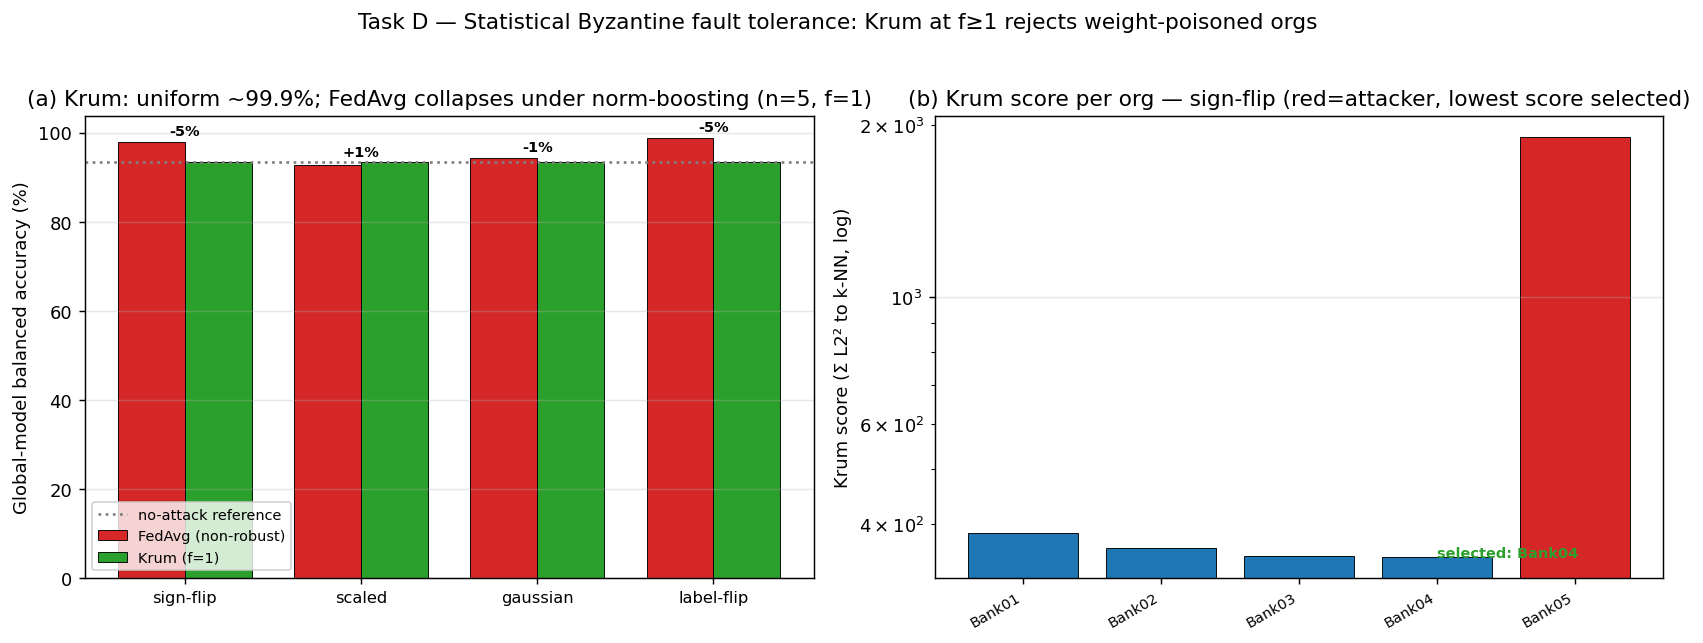
\includegraphics[width=\linewidth]{db_boa_framework/results/byzantine_robustness_krum_vs_fedavg_banksim_stratified.png}
\caption{The Byzantine layer on the control condition. \textbf{(b)} shows the security property that
replicates everywhere --- the poisoned organisation's Krum score is orders of magnitude above the
others, so it is never selected. \textbf{(a)} shows the part we had to withdraw a mechanism for: the
accuracy difference between Krum and unprotected averaging is small and mostly negative here, and it
tracks the dataset rather than the federation structure.}
\end{figure}

% =====================================================================
\section{What may be quoted, and what may not}
\label{sec:quotable}

This section exists because several numbers in older drafts and in the supervisor brief are no longer
safe. \textbf{If you are writing anything, read this list first.}

\begin{center}\small
\renewcommand{\arraystretch}{1.2}
\begin{tabularx}{\linewidth}{@{}p{5.6cm} X@{}}
\toprule
\textbf{Do not quote} & \textbf{Quote instead} \\
\midrule
``Krum pays 1.5--12.6\,pp under entity-disjointness'' & Krum rejects the attacker 8/8 in all three conditions; it can cost utility by an amount that tracks the dataset; \textbf{no mechanism is on record}. Use the \emph{clean-cell} ranges: $-4.73$ to $-1.48$\,pp (entity-disjoint), $-9.15$ to $+0.54$\,pp (stratified). \\
``a 60\x{} privacy-budget improvement'' (or 30\x, 33\x, $\ge$100\x) & The \textbf{ordering} (paired, 12/12 probed budgets) and the \textbf{$\rh$-gap at a stated $\eps$}. If a magnitude is unavoidable: ``one to two orders of magnitude, definition-sensitive''. \\
``MC-Shapley top-1 fails from $n\ge6$'' & Top-1 agreement is \textbf{intermittent, not a threshold}: 5/10, 5/10, 3/10, and it first fails at $n{=}3$ on BankSim. \\
Any number from \texttt{db\_boa\_results.json} or \texttt{baselines.json} (including MCC 0.677 as a tuned result) & \textbf{Invalid for three separate reasons} --- a search that could not rank candidates, a surrogate validating on memorised rows, and the unexplained ULB divergence. Two are fixed; the third is not. Regenerate before quoting, and scope the third explicitly. \\
MCC 0.313, 97.38\% accuracy, MCC 0.966, 85\,TPS, 180\,ms & Withdrawn before submission or during the multi-seed work. The detector headline is \textbf{0.753\,$\pm$\,0.055 over five seeds}, and Fabric is \textbf{2115.9\,ms / 40.3\,TPS}. \\
A repaired \texttt{steps\_per\_epoch} optimum as a precise value & The \emph{implied batch size}. The repaired axis yields only 23 distinct batch sizes across 201 values, and a third of the range collapses into two bins. \\
Any pre-1 September ULB result & Nothing yet --- the reproduction failure is unexplained. BankSim is unaffected; both partitions reproduced bitwise. \\
\bottomrule
\end{tabularx}
\end{center}

\begin{keybox}{Two framing rules that apply to everything above}
\textbf{Name the metric (Rule 11).} Twice in this period two metrics ranked the same cell oppositely:
Monte-Carlo rank fidelity and top-1 agreement disagree about which dataset is better, and the privacy
ordering scores 11/11 on one metric and 10/11 on the other. Stating which one you are quoting is not
pedantry --- it is the difference between a claim and a selection.

\textbf{Say ``measured on the evidence swept'', not ``measured''.} Several quantities here get larger
the harder anyone looks. That is a property of how they are defined, and it belongs next to the number.
\end{keybox}

% =====================================================================
\section{What is left, and the plan to 19 September}

\begin{center}\small
\begin{tabularx}{\linewidth}{@{}c p{4.4cm} X c@{}}
\toprule
\textbf{\#} & \textbf{Task} & \textbf{Why it is in this position} & \textbf{Cost} \\
\midrule
1 & Finish the re-runs the surrogate repair forces --- regenerate the two invalid result files on the fixed pool, then re-run the multi-seed detector with the repaired configuration as an extra arm & The multi-seed headline ($+0.047$, $p=0.34$) currently compares a \emph{noise-selected} configuration against the default. The plumbing is already done. \textbf{Read the ULB reproduction freeze first} --- a regenerated ULB number is quotable only if that third defect is addressed or explicitly scoped. & 3--5\,h \\
2 & Third dataset (Fraud Detection Handbook), \textbf{go/no-go 12 September} & Must come \emph{after} item 1, or its search arm is generated on a surrogate we already know is broken and paid for twice. & loader + $\sim$6\,h \\
3 & Formalise the DP threat model; scope the two overstated title words & Both flagged must-fix before publication. Both are writing, not code. & writing \\
\bottomrule
\end{tabularx}
\end{center}

\begin{keybox}{Two hard commitments}
\textbf{The 16--19 September writing block is protected.} If the third dataset overruns, \textbf{the
dataset is cut, not the writing}. A half-run third column is unusable \emph{and} it invites exactly the
lopsided-table criticism Rule~8 exists to prevent.

\textbf{The 12 September go/no-go is decided on the date, not on sunk cost.} If the loader is not
producing sane sweeps by then, it is dropped.
\end{keybox}

\subsection{Open questions we are carrying honestly}

\begin{enumerate}[label=\textbf{Q\arabic*.}]
  \item \textbf{Why does the 30 August ULB result not reproduce?} Everything reachable has been
  eliminated. The remaining candidate --- the numeric library version at the time --- is unrecoverable.
  Recorded as unexplained; guarded against recurrence.
  \item \textbf{Does that reproduction failure reach the detector track?} Only one sweep was
  re-verified. Every ULB number generated before 1 September sits on a code and environment state that
  no longer exists. If a detector number moved the way the contribution split did, that is a
  Chapter\,5 problem, not a paper-extension one. \emph{If nothing moved, that is a clean reproducibility
  statement worth having in writing.}
  \item \textbf{Why does Krum cost utility on BankSim?} The effect is measured and real; the mechanism
  we proposed is falsified. No replacement is on record, and inventing one would be the failure this
  whole period was about.
  \item \textbf{Should the deployed model adopt the repaired batch-size formula?} Zero CPU to decide,
  but changing it invalidates every trained model. Deliberately still open.
  \item \textbf{What do Shapley values look like under an entity-disjoint split?} Still unmeasured ---
  the current near-uniform values $[0.167, 0.165, 0.165]$ are the reason the incentive layer has little
  to attribute. Not on the locked plan; no window before the deadline.
\end{enumerate}

% =====================================================================
\section{Closing assessment}

Six days ago the work had one real contribution resting on one dataset, an unaudited search at its
centre, and a censored statistic quoted as a measurement. It now has the same contribution resting on
two datasets and three conditions, an audited search with a stronger negative result than before, and a
statistic we have deliberately stopped quoting.

Three headline claims died in the process. All three died to controls we ran on ourselves, each of
which had written down in advance what its own failure would mean. That is the difference between a
result and an objection.

\begin{keybox}{The honest summary for the supervisor}
\textbf{The work is smaller than it looked on 30 August, and considerably harder to argue with.} The
paper's contribution --- that weight-channel differential privacy destroys the contribution signal that
pays participants, and that moving the noise to the released contribution channel restores it ---
survives on two datasets and three federation conditions, and it now rests on two threshold-free
statements rather than on a ratio that moves with its own definition. Everything that did not survive
is written down as not having survived.
\end{keybox}

\newpage
% =====================================================================
\appendix
\section{Glossary}

\begin{center}\small
\renewcommand{\arraystretch}{1.2}
\begin{tabularx}{\linewidth}{@{}p{3.5cm} X@{}}
\toprule
\textbf{Term} & \textbf{Meaning in this work} \\
\midrule
\textbf{FL-ADTCN} & The whole system: federated Adaptive Deep Temporal Context Networks + differential privacy + Krum + Shapley + DB-BOA + reinforcement-learning leader election on Hyperledger Fabric. \\
\textbf{ADTCN} & Our detector. A 1-D convolutional network over a window of 10 consecutive transactions, with a pooling step over time. Measured as a component; it ranks 5th of 7 on ULB and 7th of 7 on BankSim's customer-linked windows. \\
\textbf{DB-BOA} & Dynamic Butterfly--Billiards Optimisation Algorithm, the hybrid metaheuristic from the base paper, used here to search the detector's hyperparameters. \\
\textbf{Surrogate / objective} & The small, fast model DB-BOA trains to \emph{score} a candidate configuration. Not the deployed model. Most of Section~\ref{sec:obj13} is about this distinction. \\
\textbf{Differential privacy (DP), $\eps$} & Calibrated random noise added before sharing. Smaller $\eps$ means more privacy and more noise. \\
\textbf{Weight channel vs output channel} & \emph{Where} the noise is added: to the model weights an organisation shares, or to the contribution value it publishes. The choice between these is the paper's contribution. \\
\textbf{Krum} & A rule that picks the single most ``central'' weight vector among the organisations, so an outlier or poisoned one is never used. Security, not fairness. \\
\textbf{Shapley value} & A cooperative-game measure of how much each organisation contributed, used here to split token rewards. Fairness, not security. \\
\textbf{Rank inversion} & The reward ranking coming out in the wrong order after noise --- i.e.\ someone is paid as if they contributed more than they did. \\
\textbf{\epsst} & The largest privacy budget at which a rank inversion was still \emph{caught}. Section~\ref{sec:obj17} explains why this is not a stable statistic. \\
\textbf{MCC} & Matthews correlation coefficient. The right headline metric on 0.17\%-fraud data, where accuracy is uninformative. \\
\textbf{Stratified vs entity-disjoint split} & How transactions are dealt to the three banks: by preserving the fraud ratio (volume split of one institution) versus by dealing whole \emph{customers}, so no customer's history appears in two banks. \\
\textbf{Confound control} & An extra run that changes only one factor, so an effect can be attributed. Section~\ref{sec:control}. \\
\textbf{Pre-registration} & Writing down the expected result --- and what being wrong would mean --- before the run, then scoring underneath without editing. \\
\textbf{Common random numbers} & Scoring every candidate on the \emph{same} random draws, so the comparison between them is not corrupted by draw-to-draw luck. The finding of Section~\ref{sec:obj13}. \\
\bottomrule
\end{tabularx}
\end{center}

\section{Where everything lives}

\textbf{The running state of the work} is \texttt{TASK.md} at the repository root --- objectives,
pre-registrations, scorecards, and a verified-numbers table. Start at its \textsc{resume here} section.
\textbf{Numbers live only in} \texttt{db\_boa\_framework/results/*.json}; generated write-ups live in
\texttt{final\_report\_data/}. \textbf{Never hand-edit a generated draft} --- regenerate it, which now
takes seconds.

\begin{center}\small
\begin{tabularx}{\linewidth}{@{}p{5.2cm} X@{}}
\toprule
\textbf{Script} (all under \texttt{db\_boa\_framework/experiments/}) & \textbf{Produces} \\
\midrule
\texttt{banksim\_temporal\_grid.py} & The entity-linked window grid (7 architectures $\times$ 2 orderings). \\
\texttt{basepaper\_comparison.py} & The base-paper classifier and optimiser tracks, both datasets. \\
\texttt{detector\_multiseed.py} & The 5-seed detector headline and the determinism probe. \\
\texttt{byzantine\_robustness\_sweep.py} & Krum at $n\ge2f+3$, four attack types. \\
\texttt{economic\_byzantine\_sweep.py} & Collusion, lone attackers, free-riders, isolation. \\
\texttt{private\_incentive\_sweep.py} & The privacy $\leftrightarrow$ incentive channels; takes \texttt{--eps-grid} and \texttt{--repeats}. \\
\texttt{scalability\_sweep.py} & Exact vs Monte-Carlo Shapley cost and fidelity. \\
\texttt{sweeps\_cross\_condition.py} & \textbf{The only correct way to compare conditions.} Prints dataset effect and partition effect as separate columns and marks contaminated cells. Reads JSON only; seconds. \\
\texttt{objective\_noise\_audit.py} & The surrogate diagnosis. Deliberately pins the \emph{pre-repair} behaviour. \\
\texttt{obj13\_shipped\_path\_check.py} & The check that found the memorised-rows leak. Zero training. \\
\texttt{obj13\_surrogate\_repair.py} & The three-mode side-by-side and its held-out yardstick. \\
\bottomrule
\end{tabularx}
\end{center}

\begin{keybox}{Operational notes that cost time to learn}
\textbf{Use the PowerShell runners}, not the shell scripts --- \texttt{python} is absent from Git Bash's
path on this machine and the alternative on the path has no \texttt{torch}. \textbf{Set
\texttt{PYTHONIOENCODING=utf-8}} when redirecting output, and open files with an explicit encoding ---
these are two \emph{different} traps and the first does not fix the second. \textbf{Launch multi-hour
work detached}, with a preflight that asserts the code state before spending the CPU; a preflight costing
seconds is the reason the 16-hour run held no surprises. \textbf{Every detector number requires a pinned
torch version and thread count} to mean anything.
\end{keybox}

\vfill
\begin{center}\footnotesize\color{steel}
Compiled 5 September 2026 from the repository state at branch \texttt{obj13-surrogate-repair}.\\
Every figure in this document was produced by a script in that repository.
\end{center}

\end{document}
